\documentclass{beamer}
\usepackage{risk201}

\setchapter{4}
\renewcommand{\tlsize}{\footnotesize}  % fraction labels need the larger size

\title{RISK 201: General and Other Annuities}

\begin{document}
\maketitle

%======================================================================
\section{General annuities}
%======================================================================

\begin{frame}{4.1 General annuities}

\begin{itemize}
\item An annuity for which payments are made more or less frequently than interest is compounded is called a \textbf{general annuity}.
\bigskip
\item The simplest technique to solve problems involving general annuities is to \textbf{replace the given interest rate} with an equivalent rate whose compounding period matches the payment periods.
\end{itemize}

\end{frame}

\begin{frame}{Example 4.1}

Payments of \$500 are made for two years at the beginning of each month. Find the present value of these payments if the effective annual rate is 6\%.

\bigskip
\begin{center}
\timeline{10}{0/0, 1/1, 2/2, 4.5/11, 5.5/12, 8.5/23, 9.5/24}
\end{center}

\vfill
\end{frame}

\begin{frame}{Alternative approach}

An alternative approach is to \textbf{replace the payments} with equivalent payments whose frequency matches the interest compounding period.

\bigskip
\underline{Example 4.1, continued}

\bigskip
\begin{center}
\cfdiagram{10}{0/0, 1/1, 2/2, 3.25/\cdots, 4.5/11, 5.5/12, 7/\cdots, 8.5/23, 9.5/24}{0/{$500$}, 1/{$500$}, 2/{$500$}, 3.25/{$\cdots$}, 4.5/{$500$}, 5.5/{$500$}, 7/{$\cdots$}, 8.5/{$500$}}
\end{center}

\vfill
\end{frame}

\begin{frame}{Ordinary annuity payable $m$-thly}

\begin{itemize}
\item[] $m$ = \# of payment periods in one interest conversion period,
\item[] $n$ = term of the annuity (in interest conversion periods),
\item[] $i$ = effective interest rate per period
\end{itemize}

\bigskip
Actuarial notation for present value of an annuity that pays $1/m$ at the end of each $m$-thly period for $n$ years is $a_{\angl{n}i}^{(m)}$, read as ``a upper $m$ angle $n$ at $i$''.

\end{frame}

\begin{frame}{PV of annuity payable $m$-thly}

\begin{center}
\cfdiagram{10}{0/0, 1.2/\frac{1}{m}, 2.4/\frac{2}{m}, 3.4/\cdots, 4.4/\frac{m-1}{m}, 5.6/1, 6.6/\cdots, 7.9/n-\frac{1}{m}, 9.4/n}{1.2/{$\frac{1}{m}$}, 2.4/{$\frac{1}{m}$}, 3.4/{$\cdots$}, 4.4/{$\frac{1}{m}$}, 5.6/{$\frac{1}{m}$}, 6.6/{$\cdots$}, 7.9/{$\frac{1}{m}$}, 9.4/{$\frac{1}{m}$}}
\end{center}

\[
PV = a_{\angl{n}i}^{(m)} = \frac{1-v^n}{i^{(m)}}
\]

\vfill
\end{frame}

\begin{frame}{FV of annuity payable $m$-thly}

\begin{center}
\cfdiagram{10}{0/0, 1.2/\frac{1}{m}, 2.4/\frac{2}{m}, 3.4/\cdots, 4.4/\frac{m-1}{m}, 5.6/1, 6.6/\cdots, 7.9/n-\frac{1}{m}, 9.4/n}{1.2/{$\frac{1}{m}$}, 2.4/{$\frac{1}{m}$}, 3.4/{$\cdots$}, 4.4/{$\frac{1}{m}$}, 5.6/{$\frac{1}{m}$}, 6.6/{$\cdots$}, 7.9/{$\frac{1}{m}$}, 9.4/{$\frac{1}{m}$}}
\end{center}

\[
FV = s_{\angl{n}i}^{(m)} = \frac{1-v^n}{i^{(m)}} \cdot (1+i)^n = \frac{(1+i)^n - 1}{i^{(m)}}
\]

\vfill
\end{frame}

\begin{frame}{Example 4.2}

You will receive 96 monthly payments starting one month from now. Payments are \$100 and the effective annual rate of interest is 12\%. Find the present value of this annuity today.

\bigskip
\begin{center}
\timeline{10}{0/0, 1.2/\frac{1}{12}, 2.4/\frac{2}{12}, 3.4/\cdots, 4.4/\frac{11}{12}, 5.6/1, 6.6/\cdots, 7.9/7\frac{11}{12}, 9.4/8}
\end{center}

\vfill
\end{frame}

\begin{frame}{Example 4.2, continued}

\begin{center}
\cfdiagram{10}{0/0, 1.2/\frac{1}{12}, 2.4/\frac{2}{12}, 3.4/\cdots, 4.4/\frac{11}{12}, 5.6/1, 6.6/\cdots, 7.9/7\frac{11}{12}, 9.4/8}{1.2/{$100$}, 2.4/{$100$}, 3.4/{$\cdots$}, 4.4/{$100$}, 5.6/{$100$}, 6.6/{$\cdots$}, 7.9/{$100$}, 9.4/{$100$}}
\end{center}

\vfill
\end{frame}

\begin{frame}{Annuity-due payable $m$-thly}

\begin{center}
\cfdiagram{10}{0/0, 1.2/\frac{1}{m}, 2.4/\frac{2}{m}, 3.4/\cdots, 4.4/1, 5.6/\frac{m+1}{m}, 6.6/\cdots, 7.9/n-\frac{1}{m}, 9.4/n}{0/{$\frac{1}{m}$}, 1.2/{$\frac{1}{m}$}, 2.4/{$\frac{1}{m}$}, 3.4/{$\cdots$}, 4.4/{$\frac{1}{m}$}, 5.6/{$\frac{1}{m}$}, 6.6/{$\cdots$}, 7.9/{$\frac{1}{m}$}}
\end{center}

$\ddot{a}_{\angl{n}i}^{(m)}$ is PV of annuity that pays $1/m$ at the \textbf{beginning} of each $m$-thly period for $n$ years, $\ddot{s}_{\angl{n}i}^{(m)}$ is FV
\[
\ddot{a}_{\angl{n}i}^{(m)} = \frac{1-v^n}{d^{(m)}} \qquad \text{and} \qquad \ddot{s}_{\angl{n}i}^{(m)} = \frac{(1+i)^n - 1}{d^{(m)}}
\]

\end{frame}

%======================================================================
\section{Mortgages}
%======================================================================

\begin{frame}{4.2 Mortgages}

\begin{itemize}
\item Mortgages are a special type of loan where the \textbf{property is pledged as security} in case of default (non-payment) by the borrower.
\medskip
\item In Canada, mortgages are offered by various banks, credit unions and private lenders.
\medskip
\item We distinguish between \textbf{residential mortgages} (for properties where the owners will live) and \textbf{commercial mortgages} (for properties purchased as investment). The processes and rules for issuing commercial mortgages are different from residential mortgages.
\end{itemize}

\end{frame}

\begin{frame}{Lenders}

\begin{itemize}
\item \textbf{``A'' lenders}: Mortgage lenders with strict criteria about who they lend to, heavily regulated
  \begin{itemize}
  \item The ``Big Five'' and their various brands
  \item Some smaller banks
  \item Credit unions
  \end{itemize}
\item \textbf{``B'' lenders}: mortgage lenders with less strict criteria but still regulated
\item \textbf{``C'' lenders}: private lenders, not directly regulated
\end{itemize}

\end{frame}

\begin{frame}{Regulation}

\begin{itemize}
\item Banks are regulated federally under the \textit{Bank Act} and supervised by the Office of the Superintendent of Financial Institutions (OSFI)
\medskip
\item Most credit unions are regulated provincially
\medskip
\item \textit{Interest Act} also applies: sets rules about rates and how to communicate/quote them
\end{itemize}

\end{frame}

\begin{frame}{Down payment}

\begin{itemize}
\item \textbf{Conventional mortgage}: at least 20\% down payment (loan-to-value ratio $\le$ 80\%)
\medskip
\item \textbf{High-ratio mortgages}: less than 20\% down payment (loan-to-value ratio $>$ 80\%)
\medskip
\item High-ratio mortgages will typically require mortgage default insurance
\end{itemize}

\end{frame}

\begin{frame}{Mortgage default insurance}

\begin{itemize}
\item Mortgage default insurance (aka mortgage loan insurance) protects the lender in case of default by borrower
\medskip
\item Issued by Canada Mortgage and Housing Corporation (CMHC) and a few others
\medskip
\item Only mortgages with a big enough down payment are insured by CMHC
\end{itemize}

\end{frame}

\begin{frame}{Mortgage default insurance, cont'd}

\begin{itemize}
\item Minimum down payment to qualify for mortgage insurance through CMHC: 5\% of first \$500,000 of property value, 10\% of rest
\medskip
\item CMHC does not insure mortgages on properties valued over \$1.5 / 1 million (homeowner / rental)
\medskip
\item Insurance premium is charged at issue as a \% of the mortgage amount, can be paid in cash or rolled into mortgage
\medskip
\item Typical premium is 2.4\%--4.0\%, depending on LTV
\end{itemize}

\end{frame}

\begin{frame}{Amortization period}

\begin{itemize}
\item The period over which the mortgage loan is assumed to be paid back
\item Maximum amortization period in Canada:
  \begin{itemize}
  \item For CMHC-insured mortgages: \textcolor{red}{30} years
  \item For other mortgages: 35 years
  \end{itemize}
\item A longer amortization period will:
  \begin{itemize}
  \item Reduce the amount of mortgage payments
  \item Increase the total interest paid over the life of the mortgage
  \end{itemize}
\end{itemize}

\end{frame}

\begin{frame}{Mortgage rates}

\begin{itemize}
\item Interest rates payable on mortgages vary widely depending on the type of lender, the credit-worthiness of borrower, and whether the rate is fixed or variable
\medskip
\item Expressed as a nominal rate compounded semi-annually
\medskip
\item Annual Percentage Rate (APR) also includes fees charged to issue the mortgage
\medskip
\item Posted rate vs discounted rate
\end{itemize}

\end{frame}

\begin{frame}{Fixed vs.\ variable rates}

\begin{itemize}
\item Fixed mortgage rates are locked in for the length of the mortgage term
\medskip
\item Variable rate floats with the lender's prime rate
\medskip
\item Variable rates on mortgages are generally lower than fixed rates, but borrower takes on more risk
\end{itemize}

\end{frame}

\begin{frame}{5-year fixed rates -- posted}

\begin{center}
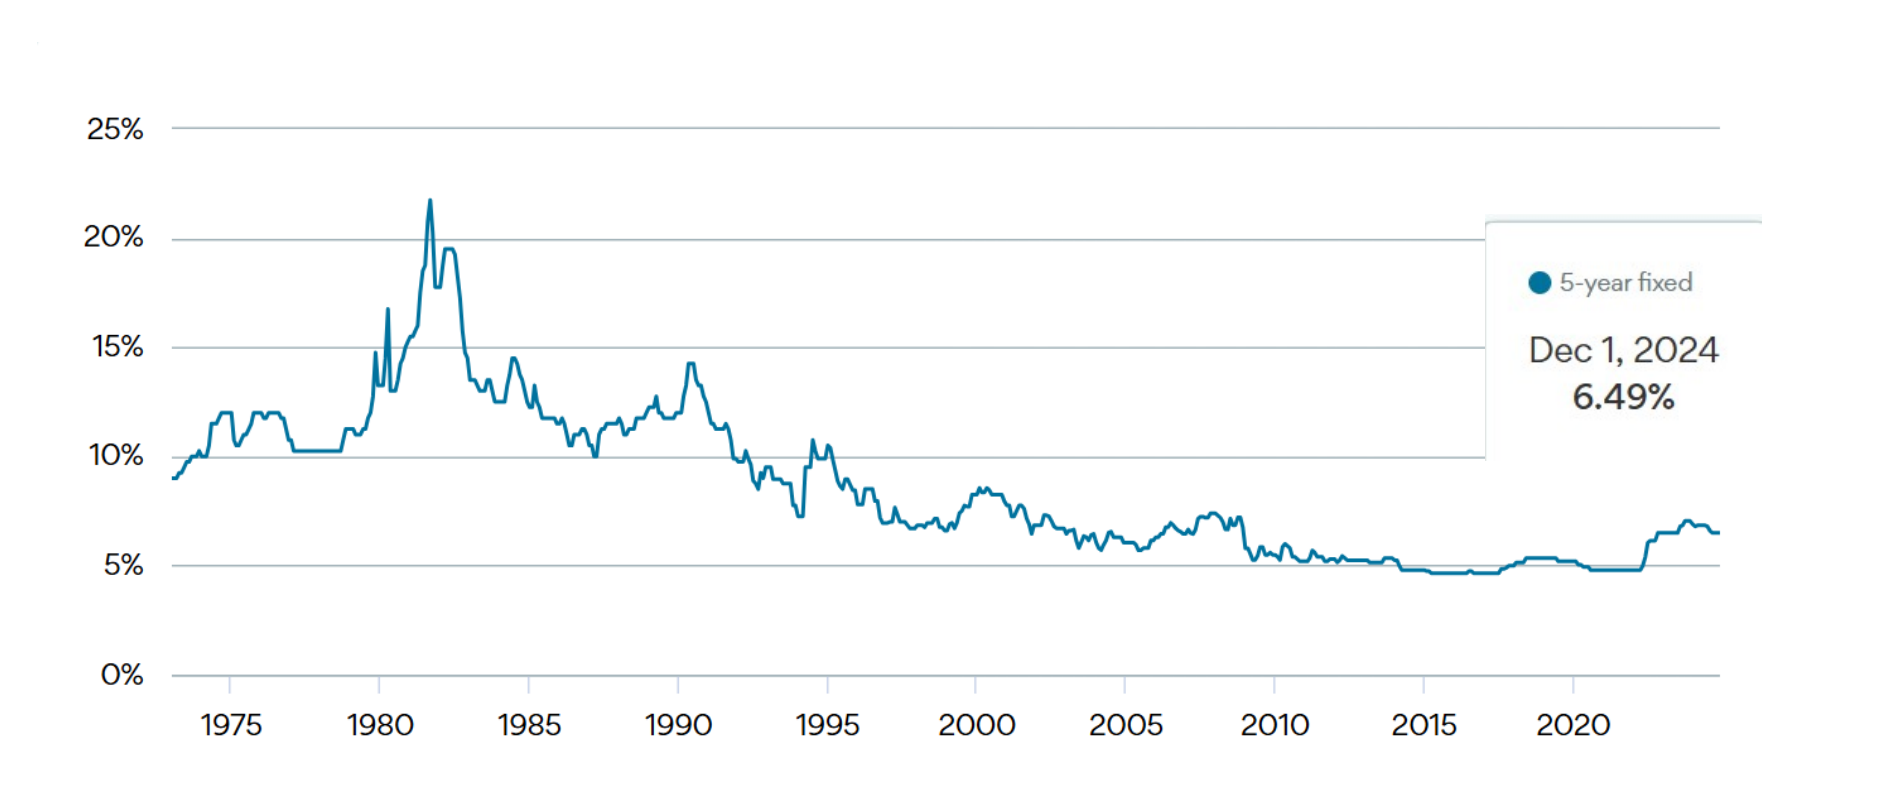
\includegraphics[width=\textwidth]{figures/ch4_fixed_posted_rates.png}

\medskip
{\scriptsize Source: \texttt{https://www.ratehub.ca/5-year-fixed-mortgage-rate-history}}
\end{center}

\end{frame}

\begin{frame}{5-year fixed rates -- discounted}

\begin{center}
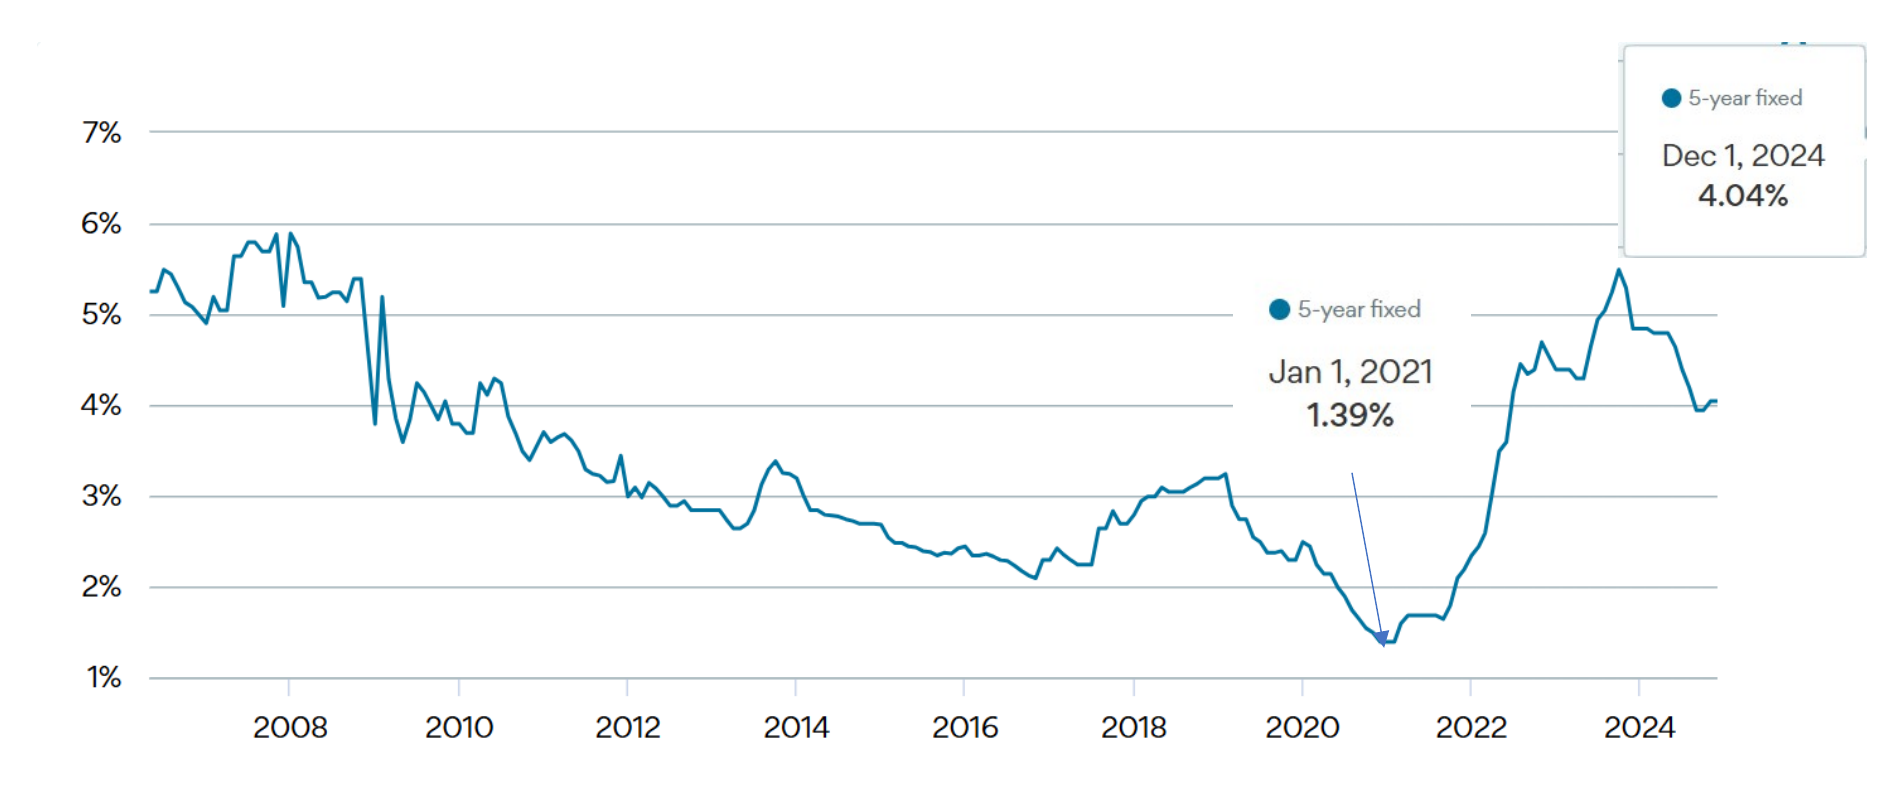
\includegraphics[width=\textwidth]{figures/ch4_fixed_discounted_rates.png}

\medskip
{\scriptsize Source: \texttt{https://www.ratehub.ca/5-year-fixed-mortgage-rate-history}}
\end{center}

\end{frame}

\begin{frame}{5-year variable rates -- discounted}

\begin{center}
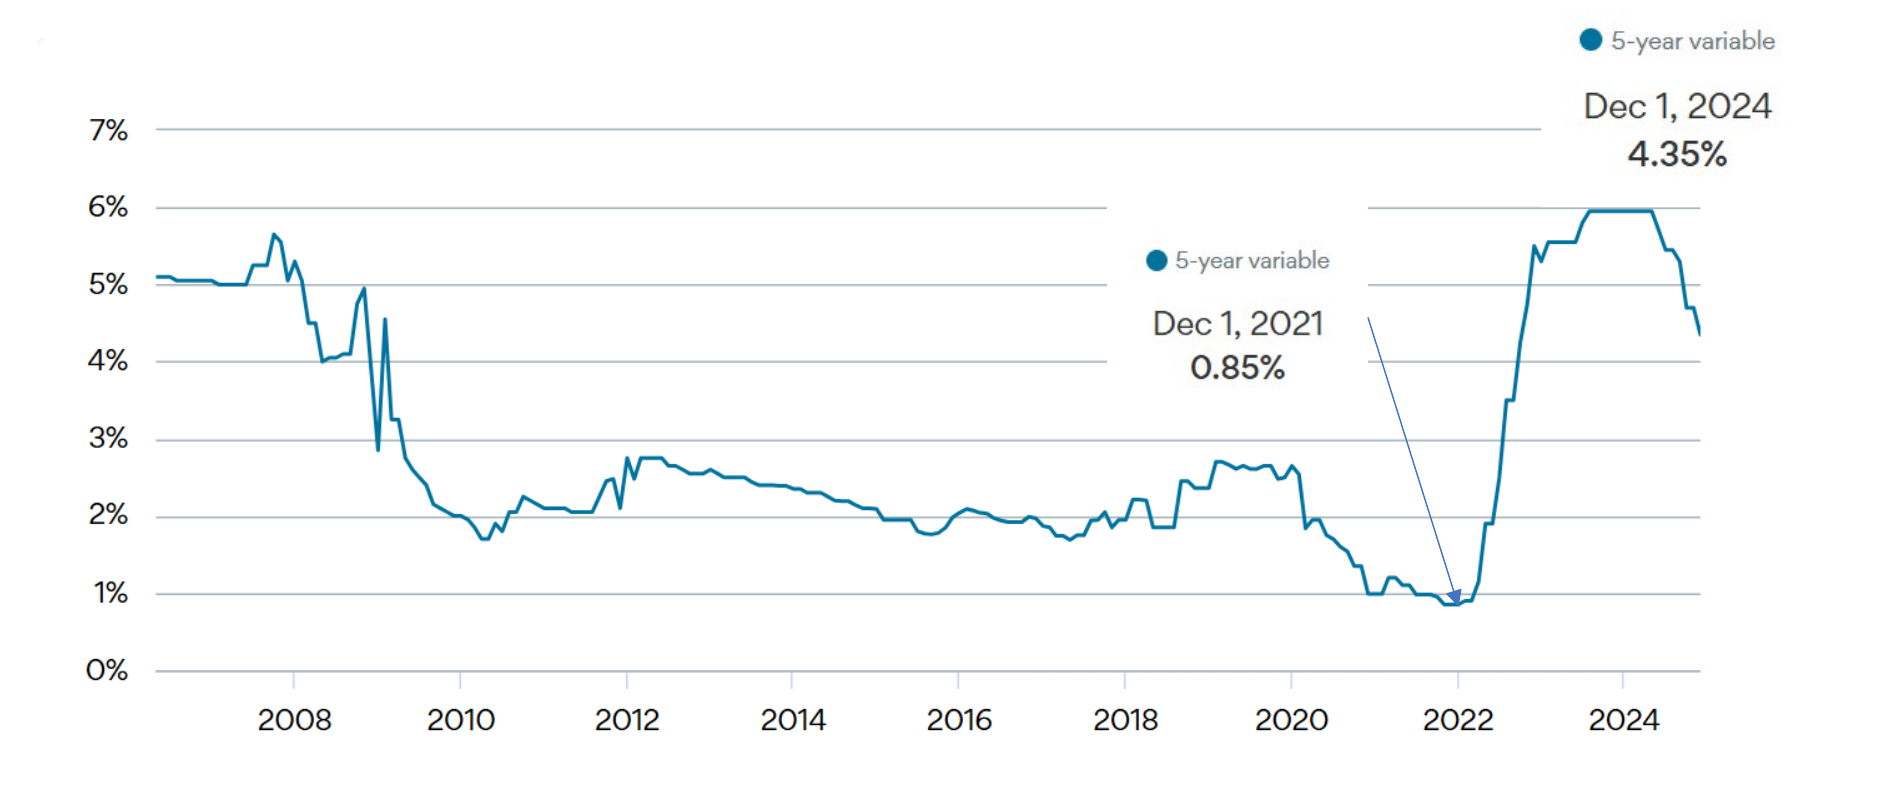
\includegraphics[width=\textwidth]{figures/ch4_variable_discounted_rates.png}

\medskip
{\scriptsize Source: \texttt{https://www.ratehub.ca/5-year-variable-mortgage-rate-history}}
\end{center}

\end{frame}

\begin{frame}{Qualifying for a mortgage}

\begin{itemize}
\item Credit score
\item Loan-to-value ratio
\item Income and debt service ratios:
  \begin{itemize}
  \item Gross debt service ratio (GDS) = PITH/gross income
  \item PITH = \textcolor{red}{\textbf{P}}rincipal, \textcolor{red}{\textbf{I}}nterest, \textcolor{red}{\textbf{T}}axes, \textcolor{red}{\textbf{H}}eat
  \item Total debt service ratio (TDS) includes all debt payments in numerator, not just the PITH associated with the mortgage
  \end{itemize}
\end{itemize}

\end{frame}

\begin{frame}{Mortgage stress testing}

\begin{itemize}
\item Introduced by OSFI \& Dept of Finance in 2012, last updated in June 2021
\item Protects stability of financial system in case of rising interest rates
\item Calculate GDS and TDS using a \textbf{qualifying interest rate}, not the contract rate
\item Current qualifying rate is 5.25\%
\item Maximum GDS = \textcolor{red}{39\%}, maximum TDS = 44\%
\end{itemize}

\end{frame}

\begin{frame}{Impact of stress test on borrowing}

\begin{itemize}
\item As the qualifying rate increases, the monthly mortgage payment that is deemed affordable decreases $\rightarrow$ reduces ability to borrow
\bigskip
\item \underline{Example 4.3}: Consider a borrower with annual household income of \$100,000 and a down payment of \$50,000, wanting a mortgage with a 25-year amortization. Ignore taxes and heating costs for simplicity.
\end{itemize}

\end{frame}

\begin{frame}{Example 4.3, continued}

\begin{center}
\footnotesize
\renewcommand{\arraystretch}{1.3}
\setlength{\tabcolsep}{4pt}
\begin{tabular}{lcc}
\toprule
 & \textbf{Before June 1, 2021} & \textbf{After June 1, 2021} \\
\midrule
Household income & \$\blue{100,000} & \$\blue{100,000} \\
Down payment & \$\blue{50,000} & \$\blue{50,000} \\
Amortization period & 25 years & 25 years \\
Qualifying rate & 4.79\% & 5.25\% \\
Maximum monthly pmt & 3,250 & 3,250 \\
 & (=\textcolor{red}{39\%}*\blue{100,000}/12) & (=\textcolor{red}{39\%}*\blue{100,000}/12) \\
Maximum mortgage & $3250\,a^{(12)}_{\angl{25}0.0479} = 573{,}643$ & $3250\,a^{(12)}_{\angl{25}0.0525} = 548{,}934$ \\
Maximum home value & 623,643 & 598,934 \\
\bottomrule
\end{tabular}
\end{center}

\vfill
\hfill{\tiny \copyright\ B. Sanders}

\end{frame}

\begin{frame}{Prepayments}

\begin{itemize}
\item The borrower may wish to pay \textbf{more} than required under the mortgage terms $\rightarrow$ \textbf{prepayment}
\item Prepayments accelerate the rate at which principal is repaid and reduce the amount of interest paid during the life of the mortgage
\item Lenders put limits on prepayments and charge penalties for prepayments in excess of these limits
  \begin{itemize}
  \item Fixed rate, closed mortgages have strictest limits
  \item Variable rate, open mortgages have no limits
  \end{itemize}
\end{itemize}

\end{frame}

\begin{frame}{Mortgage-backed securities (MBS)}

\begin{itemize}
\item The steady stream of payments from mortgage loans makes for a good investment
\item Default risk is a potential problem $\rightarrow$ pool many loans together to reduce impact of default by any one borrower
\item Lenders sell loans to organizations who will then use these as collateral for a bond issue
\item Investors who buy the bond receive monthly payments, secured by the underlying stream of mortgage payments
\end{itemize}

\end{frame}

\begin{frame}{Types of MBS}

\begin{itemize}
\item \textbf{Pass-through MBS}: payments of interest and principal are passed on to investors directly through a trust
\item \textbf{Collateralized Debt Obligations (CDOs)}: the loan pool is divided into slices (``tranches'') based on characteristics such as time to maturity, credit risk
\item Credit rating of CDOs varies widely, depending on characteristics of underlying mortgage pool
\item CDOs with bigger risk pay higher rate to investors
\end{itemize}

\end{frame}

\begin{frame}{CDO-squared}

\begin{itemize}
\item A \textbf{CDO-squared} is a CDO backed by a pool of CDOs
\item A way for banks that issue CDOs to spread around their credit risk
\item Underlying CDOs divided into tranches (again); priority of different tranches varies in case of default
\item Very opaque investment, difficult to assess actual credit risk
\end{itemize}

\end{frame}

\begin{frame}{``Underwater'' mortgages}

\begin{itemize}
\item When the value of the property is lower than the outstanding balance of the mortgage, the mortgage is said to be underwater
\item Can occur in overheated/volatile housing markets following a substantial dip in home values
\item Borrowers have incentive to default on obligations and walk away from mortgage
  \begin{itemize}
  \item ``Jingle mail'' phenomenon during US subprime mortgage crisis
  \end{itemize}
\end{itemize}

\end{frame}

\begin{frame}{The US subprime lending crisis}

\begin{itemize}
\item Low standards for underwriting, increase in housing speculation, mortgage fraud $\rightarrow$ lots of subprime mortgages being issued and packaged into MBS
\item Inflated credit ratings assigned to these MBSs by ratings agencies
\item When housing bubble burst, borrowers with underwater mortgages defaulted
\item Large number of defaults weakened the MBSs written on these pools
\end{itemize}

\end{frame}

\begin{frame}{Subprime lending crisis, cont'd}

\begin{itemize}
\item MBS values declined $\rightarrow$ banks/investors losing \$
\item Banks unable to issue more loans
  \begin{itemize}
  \item Credit spreads widened
  \item Lending ground to a halt
  \end{itemize}
\item Defaults pushed housing prices further down, throwing more fuel on the fire
\item Several US banks teetering on brink of insolvency, eventually bailed out by US government and US Federal Reserve Bank
\end{itemize}

\end{frame}

\begin{frame}{Global financial crisis (2007--2008)}

\begin{itemize}
\item Losses on MBSs and CDOs and CDO\textsuperscript{2} were spread around globally
\item Many banks both issuers of CDOs and holders of other banks' CDOs
\item Trouble at a small number of banks in the US led to contagion throughout global banking system
\item Highlighted interconnectedness of global financial system and led to regulatory focus on Systemically Important Financial Institutions (SIFI)
\end{itemize}

\end{frame}

%======================================================================
\section{Perpetuities}
%======================================================================

\begin{frame}{4.3 Perpetuities}

A perpetuity is an annuity whose payments go on \textbf{forever}.

\bigskip
\textbf{Ordinary} simple perpetuity (perpetuity-immediate):

\begin{center}
\cfdiagram{8}{0/0, 1.2/1, 2.4/2, 3.6/3, 4.8/\ldots}{1.2/{$1$}, 2.4/{$1$}, 3.6/{$1$}, 4.8/{$\ldots$}}
\end{center}

\[
PV = a_{\angl{\infty}i} = 1/i
\]

\end{frame}

\begin{frame}{PV of ordinary perpetuity}

Recall the sum of an infinite geometric series:
\[
S = a + ar + ar^2 + ar^3 + \cdots = \frac{a}{1-r}
\]

PV of ordinary perpetuity:
\[
a_{\angl{\infty}i} = 1/i
\]

Limiting case of an $n$-year annuity as $n \to \infty$:
\[
a_{\angl{\infty}i} = \lim_{n\to\infty} a_{\angl{n}i} = \lim_{n\to\infty} \frac{1-v^n}{i}
\]

\vfill
\end{frame}

\begin{frame}{Perpetuity due}

\begin{center}
\cfdiagram{8}{0/0, 1.2/1, 2.4/2, 3.6/3, 4.8/\ldots}{0/{$1$}, 1.2/{$1$}, 2.4/{$1$}, 3.6/{$1$}, 4.8/{$\ldots$}}
\end{center}

\[
PV = \ddot{a}_{\angl{\infty}i} = 1 + v + v^2 + \cdots = 1 + \frac{1}{i} = 1/d
\]

\vfill
\end{frame}

\begin{frame}{Example 4.4}

You want to establish an annual \$2000 scholarship for outstanding actuarial students. If the first scholarship payment is one year from now, how much should you set aside in an endowment fund earning 4\% effective?

\bigskip
\begin{center}
\timeline{8}{0/0, 1.2/1, 2.4/2, 3.6/3, 4.8/\ldots}
\end{center}

\vfill
\end{frame}

\begin{frame}{Practical examples of perpetuities}

\begin{columns}[T]
\begin{column}{0.68\textwidth}
\small
\begin{itemize}
\item Endowment funds
  \begin{itemize}
  \item Scholarships and bursaries
  \item Institutional funding
  \item Sovereign wealth funds
  \end{itemize}
\item `Consol' bonds (UK, US)
  \begin{itemize}
  \item Short for `consolidated annuities'
  \item Borrowing by government, promise to pay fixed \% of initial principal each year (coupon) to investor, to be redeemed when government chooses
  \item UK consol first issued in 1752, final redemption in 2015
  \end{itemize}
\item Preferred shares
\item Rental income
\end{itemize}
\end{column}
\begin{column}{0.3\textwidth}
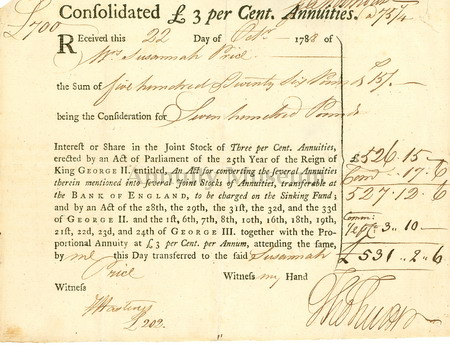
\includegraphics[width=\textwidth]{figures/ch4_consol_bond.png}
\end{column}
\end{columns}

\end{frame}

%======================================================================
\section{Continuous Annuities}
%======================================================================

\begin{frame}{4.4 Continuous Annuities}

The \textbf{present value} of an annuity making payments \textbf{continuously} at a rate of 1 per interest period for $n$ periods is denoted by $\bar{a}_{\angl{n}}$.

\begin{center}
\timeline{9}{0/0, 2.2/t, 2.9/t+dt, 4.2/1, 6.2/\ldots, 8.5/n}
\end{center}

\[
\bar{a}_{\angl{n}} = \int_0^n v^t\,dt = \int_0^n e^{-\delta t}\,dt
\]

\vfill
\end{frame}

\begin{frame}{Limit of $m$-thly ordinary annuity}

Recall that
\[
\lim_{m\to\infty} i^{(m)} = \delta.
\]

Then
\[
\bar{a}_{\angl{n}} = \frac{1-v^n}{\delta} = \lim_{m\to\infty} \frac{1-v^n}{i^{(m)}} = \lim_{m\to\infty} a_{\angl{n}}^{(m)}
\]

\end{frame}

\begin{frame}{Interpretation ($n=1$)}

\begin{center}
\begin{tikzpicture}[yscale=0.75]
  \node[anchor=east] at (-0.2,0.5) {\small Time:};
  \node at (0,0.5) {\small $0$};
  \node at (8,0.5) {\small $1$};
  \draw (0,0) -- (8,0);
  \foreach \k in {0,...,8} \draw (\k,0.12) -- (\k,-0.12);
  \node[anchor=east] at (-0.2,-1) {$a_{\angl{1}}$};
  \node[anchor=east] at (-0.2,-2) {$a_{\angl{1}}^{(2)}$};
  \node[anchor=east] at (-0.2,-3) {$a_{\angl{1}}^{(4)}$};
  \node[anchor=east] at (-0.2,-4) {$a_{\angl{1}}^{(8)}$};
  \node[anchor=east] at (-0.6,-4.9) {$\vdots$};
  \node[anchor=east] at (-0.2,-5.8) {$\bar{a}_{\angl{1}}$};
  \node at (8,-1) {$1$};
  \foreach \k in {4,8} \node at (\k,-2) {$\frac{1}{2}$};
  \foreach \k in {2,4,6,8} \node at (\k,-3) {$\frac{1}{4}$};
  \foreach \k in {1,...,8} \node at (\k,-4) {$\frac{1}{8}$};
\end{tikzpicture}
\end{center}

\end{frame}

\begin{frame}{Limit of $m$-thly annuity-due}

\[
\lim_{m\to\infty} d^{(m)} = \delta \quad\Rightarrow\quad \bar{a}_{\angl{n}} = \lim_{m\to\infty} \ddot{a}_{\angl{n}}^{(m)}
\]

\begin{center}
\begin{tikzpicture}[yscale=0.7]
  \node[anchor=east] at (-0.2,0.5) {\small Time:};
  \node at (0,0.5) {\small $0$};
  \node at (8,0.5) {\small $1$};
  \draw (0,0) -- (8,0);
  \foreach \k in {0,...,8} \draw (\k,0.12) -- (\k,-0.12);
  \node[anchor=east] at (-0.2,-1) {$\ddot{a}_{\angl{1}}$};
  \node[anchor=east] at (-0.2,-2) {$\ddot{a}_{\angl{1}}^{(2)}$};
  \node[anchor=east] at (-0.2,-3) {$\ddot{a}_{\angl{1}}^{(4)}$};
  \node[anchor=east] at (-0.2,-4) {$\ddot{a}_{\angl{1}}^{(8)}$};
  \node[anchor=east] at (-0.2,-5) {$\bar{a}_{\angl{1}}$};
  \node at (0,-1) {$1$};
  \foreach \k in {0,4} \node at (\k,-2) {$\frac{1}{2}$};
  \foreach \k in {0,2,4,6} \node at (\k,-3) {$\frac{1}{4}$};
  \foreach \k in {0,...,7} \node at (\k,-4) {$\frac{1}{8}$};
\end{tikzpicture}
\end{center}

\end{frame}

\begin{frame}{Accumulated value}

The \textbf{accumulated value} of an annuity making payments \textbf{continuously} at a rate of 1 per interest period for $n$ periods is denoted by $\bar{s}_{\angl{n}}$.

\begin{center}
\timeline{9}{0/0, 2.2/t, 2.9/t+dt, 4.2/1, 6.2/\ldots, 8.5/n}
\end{center}

\[
\bar{s}_{\angl{n}} = \int_0^n e^{\delta(n-t)}\,dt = e^{\delta n}\int_0^n e^{-\delta t}\,dt = e^{\delta n}\,\bar{a}_{\angl{n}} = \frac{(1+i)^n - 1}{\delta}
\]

\vfill
\end{frame}

\begin{frame}{Example 4.5}

\begin{itemize}
\item In 2021 and 2022 Daisy deposits \$12/day into an account.
\item The account earns interest from the exact time of the deposit, with interest quoted as an annual effective rate.
\item The rates are 9\% in 2021 and 2022.
\item Find the amount in the account, including interest, on December 31, 2022 in two ways:
\begin{itemize}
\item[(a)] exactly based on the daily deposits, and
\item[(b)] using the approximation that deposits are made continuously.
\end{itemize}
\end{itemize}

\vfill
\end{frame}

\begin{frame}{Example 4.5, continued}

Please see the Excel spreadsheet `daily, monthly, continuous annuities' file on Canvas.

\bigskip
I also recommend you try quarterly / bi-annually / usual annuities and compare their future values with given ones.

\end{frame}

\begin{frame}{Continuous annuity with varying $\delta$}

\begin{center}
\timeline{9}{0/0, 2.2/t, 2.9/t+dt, 4.2/1, 6.2/\ldots, 8.5/n}
\end{center}

\begin{align*}
\bar{a}_{\angl{n}} &= \int_0^n e^{-\int_0^t \delta_s\,ds}\,dt \\
&= \int_0^n e^{-\int_0^t \delta\,ds}\,dt = \int_0^n e^{-t\delta}\,dt = \frac{1-v^n}{\delta} \quad \text{\textcolor{red}{(if $\delta$ is constant)}} \\[1ex]
\bar{s}_{\angl{n}} &= \int_0^n e^{\int_t^n \delta_s\,ds}\,dt
\end{align*}

\end{frame}

\begin{frame}{Example 4.6 (Brown \& Kopp 4.4.A7)}

A level annuity pays \$100 per annum continuously for 20 years. If $\delta_t = \frac{1}{1+t}$, calculate the present value of this annuity.

\begin{align*}
PV = 100\,\bar{a}_{\angl{20}} &= 100\int_0^{20} e^{-\int_0^t \delta_s\,ds}\,dt = 100\int_0^{20} e^{-\int_0^t \frac{1}{1+s}\,ds}\,dt \\
&= 100\int_0^{20} e^{-\ln(t+1)}\,dt \\
&= 100\int_0^{20} 1/(t+1)\,dt = 100\ln 21
\end{align*}

\end{frame}

%======================================================================
\section{Varying annuities}
%======================================================================

\begin{frame}{4.5 Varying annuities}

In many practical situations, we have a payment stream that \textbf{varies deterministically} over time.

\medskip
We will consider three ``patterns'':
\begin{itemize}
\item Discrete payments that vary by a constant \%
  \begin{itemize}
  \item[$\rightarrow$] payments form a geometric progression
  \end{itemize}
\item Discrete payments that vary by a constant \$
  \begin{itemize}
  \item[$\rightarrow$] payments form an arithmetic progression
  \end{itemize}
\item Continuous payments that vary with time
\end{itemize}

\end{frame}

\begin{frame}{Geometric progressions}

In many situations, payments are adjusted by a \textcolor{red}{fixed percentage}:
\begin{itemize}
\item pensions adjusted for inflation,
\item wages increased according to a negotiated agreement.
\end{itemize}

\bigskip
The adjustments can happen:
\begin{itemize}
\item at the same frequency as the payments, or
\item at a different frequency.
\end{itemize}

\end{frame}

\begin{frame}{Example 4.7}

A pension plan will make annual payments starting one year from now and continuing for a total of 20 payments. The first payment will be \$24,000, with cost-of-living adjustments of 5\% per year applied to each payment thereafter. Find the present value of this pension arrangement today at an effective rate of 10\%.

\bigskip
\begin{center}
\timeline{8}{0/0, 1/1, 2/2, 3/3, 6.8/, 8/}
\end{center}

\vfill
\end{frame}

\begin{frame}{Example 4.7, continued}

\[
\begin{aligned}
\text{PV} &= v + (1+r)v^2 + (1+r)^2 v^3 + \cdots \\
&\quad + (1+r)^{n-2} v^{n-1} + (1+r)^{n-1} v^n
\end{aligned}
\]

\vspace{4em}
Where $v = \dfrac{1}{1+i}$.

\vspace{3em}
Q: What happens if $i = r$? PV $= nv$

\vfill
\end{frame}

\begin{frame}{Example 4.8}

Suppose the pension plan makes monthly payments of \$2,000 starting one month from now, up to 20 years. The payments still only increase once a year, so that the first 12 are \$2,000, the next 12 are \$2,000(1.05), and so on. Find the present value of this pension arrangement with $i^{(12)} = 5.4\%$.

\bigskip
\begin{center}
\resizebox{\textwidth}{!}{%
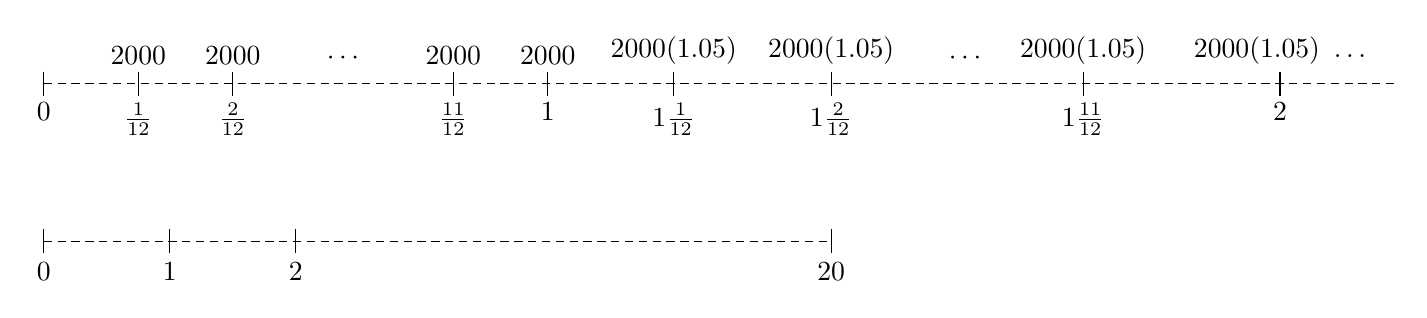
\begin{tikzpicture}
  \draw[densely dashed] (0,0) -- (17.2,0);
  \foreach \x/\t/\p in {0/0/, 1.2/\frac{1}{12}/2000, 2.4/\frac{2}{12}/2000, 3.8//\cdots, 5.2/\frac{11}{12}/2000, 6.4/1/2000, 8.0/1\frac{1}{12}/2000(1.05), 10.0/1\frac{2}{12}/2000(1.05), 11.7//\cdots, 13.2/1\frac{11}{12}/2000(1.05), 15.7/2/2000(1.05)\ \ldots} {
    \node[below] at (\x,-0.12) {$\t$};
    \node[above] at (\x,0.12) {$\p$};
  }
  \foreach \x in {0,1.2,2.4,5.2,6.4,8.0,10.0,13.2,15.7} \draw (\x,0.15) -- (\x,-0.15);
  \draw[densely dashed] (0,-2) -- (10,-2);
  \foreach \x/\t in {0/0, 1.6/1, 3.2/2, 10/20} {
    \draw (\x,-1.85) -- (\x,-2.15);
    \node[below] at (\x,-2.15) {$\t$};
  }
\end{tikzpicture}%
}
\end{center}

\vfill
\end{frame}

\begin{frame}{Arithmetic progressions}

\begin{itemize}
\item Payments are adjusted by a fixed \textbf{amount}.
\item Formulas can be derived for annuities whose payments vary in arithmetic progression:
  \begin{itemize}
  \item $n$-year increasing ordinary annuity
  \[
  PV = (Ia)_{\angl{n}i}, \quad FV = (Is)_{\angl{n}i}
  \]
  \item $n$-year decreasing ordinary annuity
  \item $n$-year increasing annuity-due
  \item $n$-year decreasing annuity-due
  \end{itemize}
\end{itemize}

\end{frame}

\begin{frame}{$n$-year increasing ordinary annuity}

\begin{center}
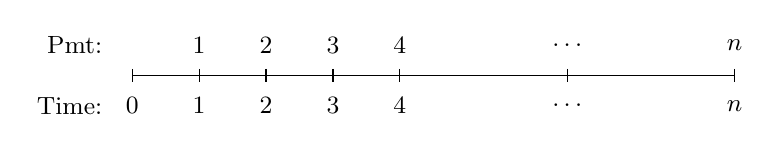
\begin{tikzpicture}[scale=0.85]
  \node[anchor=east] at (-0.3,0.45) {\small Pmt:};
  \node[anchor=east] at (-0.3,-0.45) {\small Time:};
  \draw (0,0) -- (9,0);
  \foreach \x/\t/\p in {0/0/, 1/1/1, 2/2/2, 3/3/3, 4/4/4, 6.5/\ldots/\ldots, 9/n/n} {
    \draw (\x,0.1) -- (\x,-0.1);
    \node at (\x,-0.45) {\small $\t$};
    \node at (\x,0.45) {\small $\p$};
  }
\end{tikzpicture}
\end{center}

\vspace{-1ex}
\small
\begin{align*}
(Ia)_{\angl{n}i} &= 1v + 2v^2 + 3v^3 + 4v^4 + \cdots + nv^n \\
v\,(Ia)_{\angl{n}i} &= \phantom{1v + {}} 1v^2 + 2v^3 + 3v^4 + \cdots + (n-1)v^n \textcolor{red}{{}+ nv^{n+1}} \\
(1-v)(Ia)_{\angl{n}i} &= \blue{v + v^2 + v^3 + \cdots + v^n} \textcolor{red}{{}- nv^{n+1}} = \blue{a_{\angl{n}i}} \textcolor{red}{{}- nv^{n+1}} \\
\therefore\ (Ia)_{\angl{n}i} &= \frac{a_{\angl{n}i} - nv^{n+1}}{1-v} = \frac{(a_{\angl{n}i} - nv^{n+1})(1+i)}{(1-v)(1+i)} = \frac{\ddot{a}_{\angl{n}i} - nv^n}{i} \\
(Is)_{\angl{n}i} &= (Ia)_{\angl{n}i}\,(1+i)^n = \frac{\ddot{s}_{\angl{n}i} - n}{i}
\end{align*}

\end{frame}

\begin{frame}{$n$-year decreasing ordinary annuity}

\begin{center}
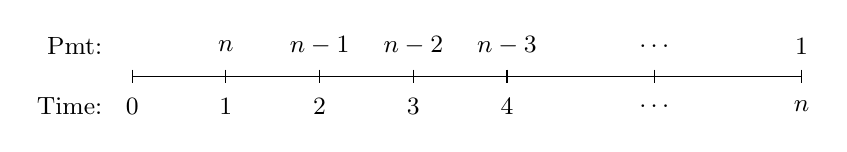
\begin{tikzpicture}[scale=0.85]
  \node[anchor=east] at (-0.3,0.45) {\small Pmt:};
  \node[anchor=east] at (-0.3,-0.45) {\small Time:};
  \draw (0,0) -- (10,0);
  \foreach \x/\t/\p in {0/0/, 1.4/1/n, 2.8/2/n-1, 4.2/3/n-2, 5.6/4/n-3, 7.8/\ldots/\ldots, 10/n/1} {
    \draw (\x,0.1) -- (\x,-0.1);
    \node at (\x,-0.45) {\small $\t$};
    \node at (\x,0.45) {\small $\p$};
  }
\end{tikzpicture}
\end{center}

\vspace{-1ex}
\small
\begin{align*}
(Da)_{\angl{n}i} &= \phantom{n + {}} nv + (n-1)v^2 + (n-2)v^3 + \cdots + 1v^n \\
\frac{1}{v}\,(Da)_{\angl{n}i} &= n + (n-1)v + (n-2)v^2 + \cdots + 1v^{n-1} \\
\frac{1-v}{v}\,(Da)_{\angl{n}i} &= n - \blue{\left(v + v^2 + \cdots + v^{n-1} + v^n\right)} = n - \blue{a_{\angl{n}i}} \\
\therefore\ (Da)_{\angl{n}i} &= \frac{v}{1-v}\left(n - \blue{a_{\angl{n}i}}\right) = \frac{n - \blue{a_{\angl{n}i}}}{i} \\
(Ds)_{\angl{n}i} &= (Da)_{\angl{n}i}\,(1+i)^n = \frac{n(1+i)^n - \blue{s_{\angl{n}i}}}{i}
\end{align*}

\end{frame}

\begin{frame}{Increasing/decreasing annuity-due}

\begin{center}
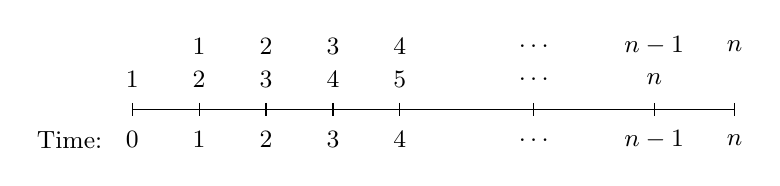
\begin{tikzpicture}[scale=0.85]
  \node[anchor=east] at (-0.3,-0.45) {\small Time:};
  \draw (0,0) -- (9,0);
  \foreach \x/\t in {0/0, 1/1, 2/2, 3/3, 4/4, 6/\ldots, 7.8/n-1, 9/n} {
    \draw (\x,0.1) -- (\x,-0.1);
    \node at (\x,-0.45) {\small $\t$};
  }
  \foreach \x/\p in {1/1, 2/2, 3/3, 4/4, 6/\ldots, 7.8/n-1, 9/n} \node at (\x,0.95) {\small $\p$};
  \foreach \x/\p in {0/1, 1/2, 2/3, 3/4, 4/5, 6/\ldots, 7.8/n} \node at (\x,0.45) {\small $\p$};
\end{tikzpicture}
\end{center}

\begin{align*}
(I\ddot{a})_{\angl{n}i} &= (Ia)_{\angl{n}i}\,(1+i) = \frac{\ddot{a}_{\angl{n}i} - nv^n}{d} \\
(I\ddot{s})_{\angl{n}i} &= (Is)_{\angl{n}i}\,(1+i) = \frac{\ddot{s}_{\angl{n}i} - n}{d} \\
(D\ddot{a})_{\angl{n}i} &= (Da)_{\angl{n}i}\,(1+i) = \frac{n - a_{\angl{n}i}}{d} \\
(D\ddot{s})_{\angl{n}i} &= (Ds)_{\angl{n}i}\,(1+i) = \frac{n(1+i)^n - s_{\angl{n}i}}{d}
\end{align*}

\end{frame}

\begin{frame}{Example 4.9}

You bought a perpetuity-due with annual payments starting at \$50 and increasing by \$50 each year until the payment amount reaches \$1000. The payments stay at \$1000 thereafter. The effective annual interest rate is 7.5\%. Find the PV of this perpetuity.

\bigskip
\begin{center}
\timeline{8}{0/0, 1/1, 2/2, 3/3, 4.5/\ldots, 6.2/, 7/}
\end{center}

\vfill
\end{frame}

\begin{frame}{Continuously varying annuities}

The present value of an $n$-year annuity for which payments are made continuously at a rate of $t$ at time $t$ is denoted by $(\bar{I}\bar{a})_{\angl{n}i}$. The accumulated value at the end of the $n$-year period is denoted by $(\bar{I}\bar{s})_{\angl{n}i}$.
\begin{align*}
(\bar{I}\bar{a})_{\angl{n}i} &= \frac{\bar{a}_{\angl{n}i} - nv^n}{\delta} \\[1ex]
(\bar{I}\bar{s})_{\angl{n}i} &= \frac{\bar{s}_{\angl{n}i} - n}{\delta}
\end{align*}

\end{frame}

\begin{frame}{General continuous annuities}

Suppose payments are made continuously for $n$ years at rate $f(t)$ at time $t$, with force of interest $\delta_t$.
\begin{align*}
\text{PV} &= \int_0^n f(t)\cdot e^{-\int_0^t \delta_s\,ds}\,dt \\
&= \int_0^n f(t)\cdot e^{-\delta t}\,dt \quad \text{\textcolor{red}{(if $\delta$ is constant)}} \\[1ex]
\text{AV} &= \int_0^n f(t)\cdot e^{\int_t^n \delta_s\,ds}\,dt \\
&= \int_0^n f(t)\cdot e^{\delta(n-t)}\,dt \quad \text{\textcolor{red}{(if $\delta$ is constant)}}
\end{align*}

\end{frame}

\begin{frame}{Example 4.10}

Deposits are being made into a fund continuously at an annual rate of \textcolor{orange}{$200e^t$} at time $t$.
\begin{enumerate}[a)]
\item Find the present value of 5 years of payments if interest is credited at \textcolor{orange}{6\%} per year compounded continuously.
\end{enumerate}

\medskip
{\small \textcolor{orange}{$f(t) = 200e^t,\ \delta = 6\%$}}

\vfill
\end{frame}

\begin{frame}{Example 4.10, continued}

\begin{enumerate}[a)]
\setcounter{enumi}{1}
\item What is the accumulated value of the fund at the end of the third year?
\end{enumerate}

\vfill
\end{frame}

\end{document}
